%=====================================================================
\section{RL baseline against the MILP}

\subsection{Valid plans, cost and speed}

\begin{table}[H]
\centering
\caption{RL baseline against the MILP baseline, by class. Gap = $100\,(Z_{\text{RL}}-Z_{\text{MILP}})/Z_{\text{MILP}}$ over instances where both plans are valid; s = mean seconds per instance.}
\small
\begin{adjustbox}{max width=\linewidth}
\begin{tabular}{@{}lrrrrrrr@{}}
\toprule
class & instances & MILP valid & RL valid & \shortstack{gap mean\\(\%)} & \shortstack{gap median\\(\%)} & MILP s & RL s \\
\midrule
C1 & 90 & 89 & 90 & 0.84 & 0.84 & 110 & 0.12 \\
C2 & 80 & 79 & 79 & 1.66 & 1.80 & 109 & 0.12 \\
R1 & 120 & 75 & 89 & 0.38 & 0.31 & 137 & 0.12 \\
R2 & 110 & 110 & 110 & 1.16 & 1.26 & 130 & 0.12 \\
RC1 & 80 & 42 & 52 & 0.12 & 0.33 & 171 & 0.12 \\
RC2 & 80 & 79 & 80 & 0.48 & 0.46 & 189 & 0.12 \\
\midrule
all & 560 & 474 & 500 & 0.85 & 0.76 & 140 & 0.12 \\
\bottomrule
\end{tabular}
\end{adjustbox}

\end{table}

\begin{itemize}
  \item \textbf{RL finds more valid plans}: \frlValid{} instances against the MILP's \fmilpValid. In \frlOnly{} instances RL has a valid plan where the MILP found none in 300 seconds (all of them ``time limit without a plan'' for the MILP); the reverse happens \fmilpOnly{} times. The \frlInvalid{} RL plans that are not valid include the \fmilpInfeasible{} provably infeasible instances, where no method can succeed.
  \item \textbf{RL plans cost a little more}: on the \frlPaired{} instances where both are valid, \frlGapMean\,\% more on average (median \frlGapMedian\,\%); against the instances the MILP proved optimal, \frlGapOpt\,\%. In \frlBetter{} instances RL is \emph{cheaper} than the MILP's time-limited plan.
  \item \textbf{RL is about a thousand times faster}: \frlSolveMean{} s per instance for 520 plans, against \fmilpSolveMean{} s for the MILP.
  \item \textbf{Where RL is closest}: the hard short-period classes R1 (0.38\,\%) and RC1 (0.12\,\%), exactly where the MILP struggles. \textbf{Where it is furthest}: C2 (1.66\,\%), long periods with clustered customers, where there are many possible orders and the MILP has time to find very good ones.
\end{itemize}

\begin{figure}[H]
\centering
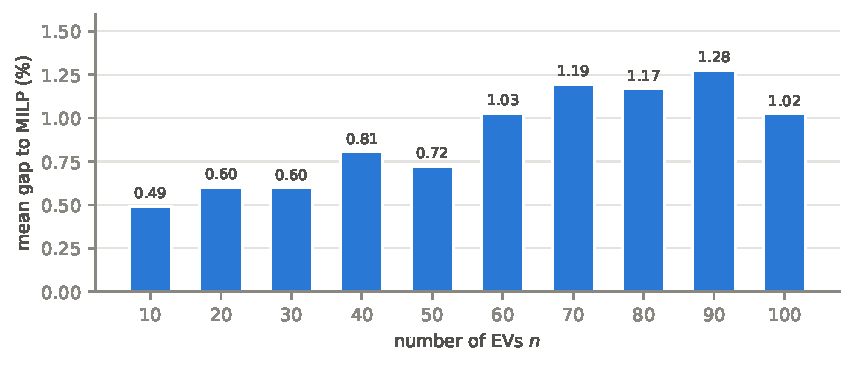
\includegraphics[width=0.85\textwidth]{figures/rl_gap_by_n.pdf}
\caption{Mean gap of RL to the MILP by instance size.}
\label{fig:rlgapn}
\end{figure}

The gap grows with size, from about 0.5\,\% at 10 cars to 1.2--1.3\,\% at 70--90 cars, and falls at 100 cars, where the MILP itself often stops far from optimal.

\inshort{RL gives a valid plan more often than the MILP, costs less than 1\,\% more on average, and needs a tenth of a second instead of more than two minutes.}

\subsection{Checks of the RL results}

All 31 RL runs (baseline + 15 variants $\times$ zero-shot and retrained) were checked file by file after the results were copied from the server:
\begin{itemize}
  \item every run has all 560 instances, each once, and no run ended with an error;
  \item a plan is marked valid exactly when it has no unplaced car and no violated rule;
  \item no RL plan is valid on an instance the MILP proved infeasible (that would be impossible);
  \item \code{plan.csv} has one row for every car of every instance;
  \item the comparison tables written on the server were recomputed from \code{runs.csv}: paired instances and mean change of $Z$ match exactly in all 30 experiment runs;
  \item an RL plan can never be cheaper than a proven optimum. Gurobi calls a plan optimal when it is within 0.01\,\% of the best possible; in 4 small instances (EV-C102 and EV-C103, 10--20 cars, in three variants) an RL plan is 0.0002--0.008\,\% cheaper than the MILP's ``optimal'' plan, i.e.\ inside that tolerance. Nowhere else;
  \item all 16 RL models are present; every training stopped early by the rule (epoch 210 or 211), with the best epoch between 145 and 201.
\end{itemize}

\inshort{The RL results are complete and consistent; the only oddity, four plans a hair cheaper than Gurobi's ``optimal'', is explained by Gurobi's 0.01\,\% optimality tolerance.}

\subsection{How RL's plans differ: it uses fewer vans}

The segment table of Part IV (and Figure~\ref{fig:vanincome}) shows the main difference in behaviour:
\begin{itemize}
  \item RL gives a van to only \fvanPersRl\,\% of free-choice personal cars, against \fvanPersMilp\,\% in the MILP plans; in the richest band 13\,\% against 41\,\%.
  \item The order is the same as the MILP's (van use rises with income for personal cars, almost zero for commercial cars), but much weaker.
  \item In exchange RL's customers queue longer at stations (commercial 3.4 against 1.6 minutes, personal 0.8 against 0.4).
\end{itemize}
Yet the cost is less than 1\,\% higher. So the cost is ``flat'' around the best plan: for a rich private owner, the van's advantages (no drive, faster charging, driver free) and its disadvantages (van premium, dearer van energy, dispatch cost) nearly balance, and moving such a customer from a van to a station changes $Z$ only a little.

Why does RL open fewer vans? Three likely reasons:
\begin{enumerate}
  \item \textbf{The dispatch cost comes first.} In the step-by-step construction, the first car put on a van carries the whole dispatch cost (Rs 1\,500) at that moment; the next five cars on the same van come almost free. The MILP sees the whole route at once. A policy that decides one car at a time sees opening a van as expensive.
  \item \textbf{Its teacher prefers stations.} The warm-up copies the greedy rule, which gives every car its cheapest option at that moment, usually a station.
  \item \textbf{Filling a van takes a coordinated series of choices}, which random sampling during training rarely finds.
\end{enumerate}
The same pattern was found for RL1 in formulation 3 (van share 3.6\,\% against the MILP's 7.0\,\%).

\inshort{RL reaches almost the same cost with a different plan: fewer vans, longer queues. This shows that many quite different plans are nearly equally good, and that RL's step-by-step view under-values opening a van.}

%=====================================================================
\section{RL experiments}

The RL rows are in the experiment tables of Part IV (Section~\ref{sec:milpexp}). Table~\ref{tab:expsummary} collects them.

\begin{table}[H]
\centering
\caption{All 15 variants: mean change of $Z$ (\%) with the MILP, RL zero-shot (ZS) and RL retrained (RT); valid plans; mean gap of RL to the MILP of the same variant (\%); training minutes and best epoch of the retrained model.}
\label{tab:expsummary}
\footnotesize
\begin{adjustbox}{max width=\linewidth}
\begin{tabular}{@{}lrrrrrrrrr@{}}
\toprule
variant & \shortstack{$\Delta Z$\\MILP} & \shortstack{$\Delta Z$\\RL-ZS} & \shortstack{$\Delta Z$\\RL-RT} & valid MILP & valid RL-RT & gap RL-ZS & gap RL-RT & train (min) & best epoch \\
\midrule
E5\_cC1\_personal\_7.5 & $-$2.21 & $-$2.49 & $-$2.46 & 473 & 500 & 0.56 & 0.56 & 38 & 201 \\
E5\_cC1\_personal\_12.5 & $+$2.08 & $+$2.45 & $+$2.38 & 473 & 500 & 1.22 & 1.14 & 39 & 200 \\
E5\_omega1\_commercial\_4.5 & $-$2.67 & $-$2.72 & $-$2.52 & 472 & 500 & 0.82 & 0.98 & 40 & 145 \\
E5\_omega1\_commercial\_7.5 & $+$2.66 & $+$2.72 & $+$2.75 & 475 & 499 & 0.83 & 0.86 & 39 & 148 \\
E6\_mu0\_personal\_1.125 & $-$1.35 & $-$1.28 & $-$1.22 & 473 & 501 & 0.92 & 0.95 & 39 & 188 \\
E6\_mu0\_personal\_1.875 & $+$1.33 & $+$1.29 & $+$1.36 & 475 & 499 & 0.80 & 0.84 & 40 & 180 \\
E6\_mu0\_commercial\_1.125 & $-$6.38 & $-$6.31 & $-$6.25 & 475 & 500 & 0.87 & 0.91 & 39 & 183 \\
E6\_mu0\_commercial\_1.875 & $+$6.43 & $+$6.34 & $+$6.33 & 475 & 500 & 0.80 & 0.79 & 38 & 200 \\
E1\_pM\_15 & $-$4.19 & $-$3.74 & $-$3.78 & 471 & 499 & 1.31 & 1.25 & 39 & 186 \\
E1\_pM\_35 & $+$3.91 & $+$3.64 & $+$3.73 & 477 & 500 & 0.58 & 0.64 & 40 & 148 \\
E2\_vans\_3 & $-$0.04 & $+$0.02 & $+$0.09 & 441 & 466 & 0.91 & 0.96 & 38 & 186 \\
E2\_vans\_7 & $+$0.02 & $+$0.04 & $+$0.00 & 487 & 506 & 0.84 & 0.81 & 38 & 181 \\
E2\_seats\_4 & $+$1.08 & $+$0.91 & $+$0.88 & 471 & 494 & 0.69 & 0.65 & 40 & 188 \\
E2\_seats\_8 & $-$0.08 & $-$0.08 & $+$0.07 & 471 & 499 & 0.85 & 0.98 & 38 & 162 \\
E8\_battery\_200 & $-$0.01 & $-$0.02 & $-$0.07 & 476 & 500 & 0.83 & 0.77 & 39 & 197 \\
\bottomrule
\end{tabular}
\end{adjustbox}

\end{table}

\subsection{Does RL measure the same effects as the MILP?}

\begin{figure}[H]
\centering
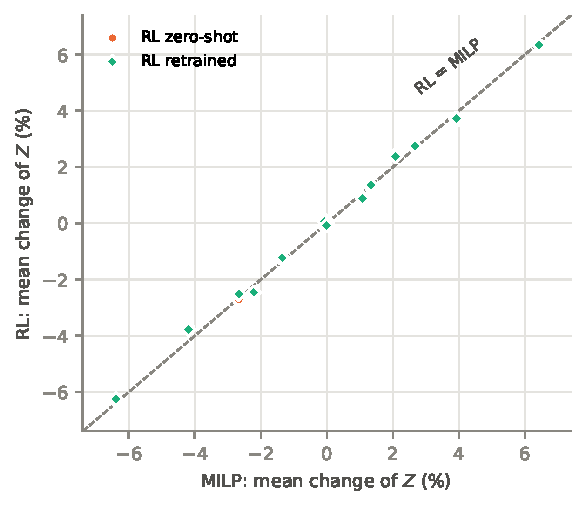
\includegraphics[width=0.55\textwidth]{figures/exp_agreement.pdf}
\caption{Change of $Z$ in each variant: MILP (horizontal) against RL (vertical). Points on the dashed line mean that RL measures exactly the MILP's effect.}
\label{fig:agree}
\end{figure}

\textbf{Yes, for the cost.} All points lie close to the line. On average the RL effect differs from the MILP effect by \fagreeZsMean{} percentage points (zero-shot) and \fagreeRtMean{} points (retrained). The direction agrees in \fagreeSign{} of \fnVariants{} variants; the two exceptions (3 vans, 8 seats) are the variants where the MILP effect itself is below 0.1\,\%, i.e.\ noise. The ranking of the assumptions (Figure~\ref{fig:tornado}) is the same with both methods.

\subsection{Does RL change who gets vans the same way?}

\begin{figure}[H]
\centering
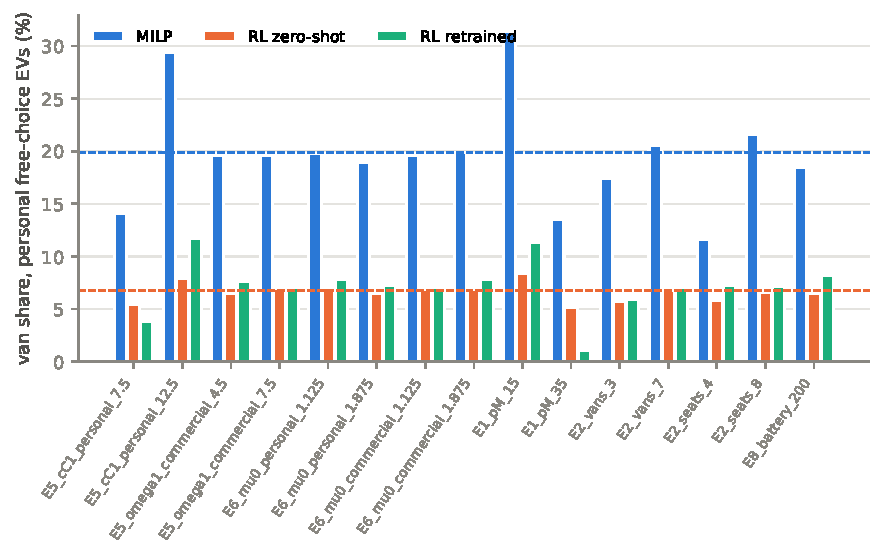
\includegraphics[width=0.95\textwidth]{figures/exp_vanshare.pdf}
\caption{Van share of free-choice personal cars in every variant. Dashed lines: the baselines (blue MILP, orange RL).}
\label{fig:expvan}
\end{figure}

\textbf{Only partly.} RL starts from a much lower van share (6.7\,\% against 19.9\,\%) and its response is weaker:
\begin{itemize}
  \item \textbf{E1 tariff}: no premium raises RL's personal van share to 8.4\,\% (zero-shot) or 11.3\,\% (retrained), the MILP's to 31.4\,\%; a doubled premium lowers it to 5.1\,\% or 1.1\,\% (MILP 13.5\,\%). Same direction, smaller size; the retrained policy reacts more than the zero-shot one.
  \item \textbf{E5 personal value of station time}: same direction (retrained 3.9\,\% and 11.7\,\%, MILP 14.1\,\% and 29.4\,\%).
  \item \textbf{E2 seats}: with 4 seats the MILP's van share falls from 19.8 to 11.6\,\%, RL's hardly moves: RL uses so few vans that the seat limit rarely binds for it.
  \item \textbf{E6 and commercial E5}: the MILP's van share does not move; the retrained policies vary by about $\pm1$ point around their baseline, which is training noise.
\end{itemize}

\subsection{Feasibility and quality in the variants}

\begin{figure}[H]
\centering
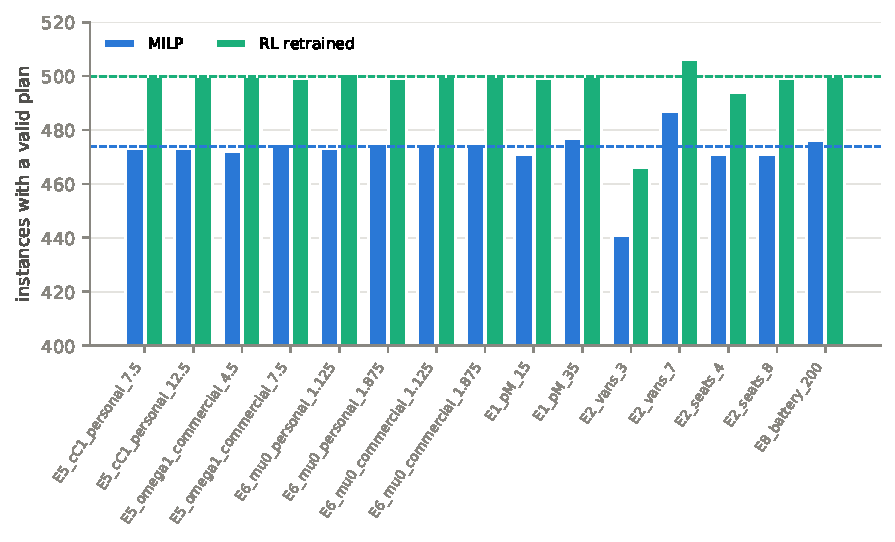
\includegraphics[width=0.95\textwidth]{figures/exp_valid.pdf}
\caption{Instances with a valid plan in every variant (dashed: the baselines).}
\label{fig:expvalid}
\end{figure}

\begin{itemize}
  \item RL has more valid plans than the MILP in every variant (465--506 against 441--487).
  \item The fleet effect is the same for both: with 3 vans RL loses 34--35 instances (MILP 33), with 7 vans it gains 6 (MILP 13).
  \item The gap to the MILP of the same variant stays between 0.56\,\% and 1.31\,\%. It is largest when vans become cheap (E1 $p^M=15$: 1.25--1.31\,\%) and smallest when they become less attractive (E5 personal 7.5: 0.56\,\%; E1 $p^M=35$: 0.58--0.64\,\%). This fits the explanation above: RL's weakness is opening vans, so it costs most when vans are worth most.
\end{itemize}

\subsection{Zero-shot or retrain?}

The zero-shot runs (baseline policy, no new training) are as good as the retrained ones: the gaps to the MILP differ by at most 0.16 points, and the measured effects on $Z$ by at most 0.2 points. Retraining took about 39 minutes per variant (15 models, best epochs 145--201). For $\pm25$\,\% changes of the customer numbers, tariff or fleet, \textbf{one trained policy can be reused without retraining}, because its inputs already contain the changed costs and fleet.

\inshort{RL measures the same cost effects as the MILP, within about 0.15 points, and keeps finding valid plans in every variant. It reacts to changes in van use in the right direction but much more weakly, because it opens few vans to begin with. Retraining is not needed for changes of this size.}
